\documentclass{beamer}

\usepackage[T1,T2A]{fontenc}
\usepackage[utf8]{inputenc}
\usepackage[english,russian]{babel}
\usepackage{tempora}

\usepackage[auto]{contour}
\usepackage{amsmath}
\usepackage{array}
\usepackage{booktabs}
\usepackage{graphicx}
\usepackage{listings}
\usepackage{ragged2e}
\usepackage{tikz}
\usepackage{xcolor}
\usetikzlibrary{arrows.meta}

\definecolor{iu9dept}{RGB}{40,40,60}
\definecolor{iu9shade}{RGB}{245,245,255}

\newcommand{\iutitle}[1]{\contour[10]{iu9shade}{\textcolor{iu9dept}{#1}}}
\newcommand{\iutitleupd}[1]{\contour[10]{iu9shade!90!gray}{\textcolor{iu9dept}{#1}}}

\newcommand{\sqlkw}[1]{\texttt{#1}}
\newcommand{\SELECT}{\sqlkw{SELECT}}
\newcommand{\FROM}{\sqlkw{FROM}}
\newcommand{\WHERE}{\sqlkw{WHERE}}
\newcommand{\JOIN}{\sqlkw{JOIN}}
\newcommand{\GROUPBY}{\sqlkw{GROUP BY}}
\newcommand{\ORDERBY}{\sqlkw{ORDER BY}}
\newcommand{\Sort}{\sqlkw{Sort}}
\newcommand{\HashJoin}{\sqlkw{HashJoin}}
\newcommand{\MergeJoin}{\sqlkw{MergeJoin}}
\newcommand{\NestedLoopJoin}{\sqlkw{NestedLoopJoin}}
\newcommand{\SeqScan}{\sqlkw{SeqScan}}
\newcommand{\IndexScan}{\sqlkw{IndexScan}}
\newcommand{\Sel}[2]{\sigma_{#1}(#2)}
\newcommand{\Projection}[2]{\pi_{#1}(#2)}
\newcommand{\Agg}[3]{\gamma_{#1;\,#2}(#3)}
\newcommand{\InnerJoin}[3]{#1 \bowtie_{#2} #3}
\newcommand{\CProd}[2]{#1 \times #2}

\lstdefinestyle{sqlstyle}{
  basicstyle=\ttfamily\footnotesize,
  columns=fullflexible,
  breaklines=true,
  keepspaces=true,
  showstringspaces=false
}
\lstset{style=sqlstyle}

\usetheme{IU9light}

\title[Автоматическая оптимизация планов выполнения SQL-запросов]{Автоматическая оптимизация планов выполнения SQL-запросов}
\date[17.06.2026]{17.06.2026}
\author[Старовойтов А.И.]{Старовойтов А.И.}
\supervisor{Руководитель: Непейвода А.Н.}
\institute{\contourlength{0.05em}\iutitle{МГТУ им. Н.Э. Баумана}\\\vspace*{-2ex}\\ \iutitle{Кафедра <<Теоретическая информатика}\\
\iutitleupd{\qquad\qquad\qquad\qquad и компьютерные технологии>>}}

\setbeamertemplate{blocks}[rounded][shadow=true]

\begin{document}

\begin{frame}[plain]
\titlepage
\end{frame}

\begin{frame}{Актуальность}
\begin{block}{Оптимизатор запросов}
Компонент СУБД, который преобразует декларативный SQL-запрос в физический план
исполнения.
\end{block}

\begin{itemize}
  \item Один SQL-запрос допускает множество эквивалентных планов.
  \item Разные порядки соединений и физические операторы дают различную стоимость.
  \item Поиск оптимального плана является NP-полной задачей в общем случае.
  \item Выбор неудачного плана может увеличить время выполнения на порядки.
\end{itemize}
\end{frame}

\begin{frame}{Цель и задачи}
\begin{block}{Цель}
Разработать и реализовать оптимизатор подмножества SQL-запросов на основе
архитектуры Cascades, а также создать каркас для его итеративного улучшения.
\end{block}

\begin{itemize}
  \item Формализовать поддерживаемое подмножество SQL и реляционной алгебры.
  \item Реализовать Memo и алгоритм поиска физического плана.
  \item Разработать правила трансформации и реализации операторов.
  \item Реализовать стоимостную модель и метод ветвей и границ.
  \item Сравнить пространство поиска с планами Microsoft SQL Server.
\end{itemize}
\end{frame}

\begin{frame}{Эффект выбора плана}
\centering
\scriptsize
\resizebox{0.94\textwidth}{!}{%
\begin{tikzpicture}[
  node distance=0.55cm,
  op/.style={rectangle, draw, fill=gray!10, rounded corners=2pt,
             text width=2.45cm, minimum height=0.72cm, align=center},
  rel/.style={rectangle, draw, rounded corners=2pt,
              text width=1.55cm, minimum height=0.54cm, align=center},
  edge/.style={->, thick}
]
  \node[font=\bfseries] at (-3.1, 3.55) {Наивный план};
  \node[op]  (nproj) at (-3.1, 2.70) {\(\pi_{\texttt{ename}}\)\\card=20\\cost=50\,050};
  \node[op]  (nfilter2) at (-3.1, 1.25) {\(\sigma_{\texttt{dname}=\texttt{'Toy'}}\)\\card=20\\cost=50\,050};
  \node[op]  (nfilter1) at (-3.1, -0.20) {\(\sigma_{\texttt{Emp.did}=\texttt{Dept.did}}\)\\card=10\,000\\cost=50\,050};
  \node[op]  (ncross) at (-3.1, -1.90) {NestedLoop\\CrossJoin\\card=\(5\cdot10^6\)\\cost=50\,050};
  \node[rel] (nemp) at (-4.55, -3.25) {\texttt{Emp}\\card=10\,000};
  \node[rel] (ndept) at (-1.65, -3.25) {\texttt{Dept}\\card=500};

  \draw[edge] (nemp) -- (ncross);
  \draw[edge] (ndept) -- (ncross);
  \draw[edge] (ncross) -- (nfilter1);
  \draw[edge] (nfilter1) -- (nfilter2);
  \draw[edge] (nfilter2) -- (nproj);

  \node[font=\bfseries] at (3.1, 3.25) {Оптимизированный план};
  \node[op]  (oproj) at (3.1, 2.45) {\(\pi_{\texttt{ename}}\)\\card=20\\cost=26};
  \node[op]  (ojoin) at (3.1, 0.85) {Index\\NestedLoopJoin\\card=20\\cost=26};
  \node[rel] (oemp) at (1.55, -0.55) {\texttt{Emp}\\card=10\,000};
  \node[op]  (ofilter) at (4.65, -0.55) {\(\sigma_{\texttt{dname}=\texttt{'Toy'}}\)\\card=1\\cost=3};
  \node[rel] (odept) at (4.65, -1.75) {\texttt{Dept}\\card=500};

  \draw[edge] (oemp) -- (ojoin);
  \draw[edge] (ofilter) -- (ojoin);
  \draw[edge] (ojoin) -- (oproj);
  \draw[edge] (odept) -- (ofilter);
\end{tikzpicture}
}
\end{frame}

\begin{frame}[fragile]{Поддерживаемое подмножество SQL}
\begin{lstlisting}
SELECT projection
FROM tables
JOIN ... ON predicate
WHERE predicate
GROUP BY attributes
ORDER BY attributes
\end{lstlisting}

\begin{itemize}
  \item Основа грамматики: диалект PostgreSQL.
  \item Поддержаны \SELECT, \FROM, \WHERE, \JOIN, \GROUPBY, \ORDERBY.
  \item Соединения: \sqlkw{INNER}, \sqlkw{LEFT}, \sqlkw{RIGHT}, \sqlkw{FULL}, \sqlkw{CROSS}.
  \item Агрегации: \sqlkw{SUM}, \sqlkw{COUNT}, \sqlkw{COUNT(*)}.
  \item Предикаты: сравнения, \sqlkw{AND}, \sqlkw{OR}, \sqlkw{NOT}, \sqlkw{BETWEEN}, \sqlkw{IN}, проверки \sqlkw{NULL}.
\end{itemize}
\end{frame}

\begin{frame}{Cascades и Memo}
\begin{columns}[T,onlytextwidth]
\begin{column}{0.49\textwidth}
\begin{itemize}
  \item Cascades хранит пространство поиска в структуре Memo.
  \item Группа Memo объединяет логически эквивалентные выражения.
  \item Групповое выражение содержит оператор и ссылки на дочерние группы.
  \item Поиск управляется стеком задач.
\end{itemize}
\end{column}
\begin{column}{0.49\textwidth}
\centering
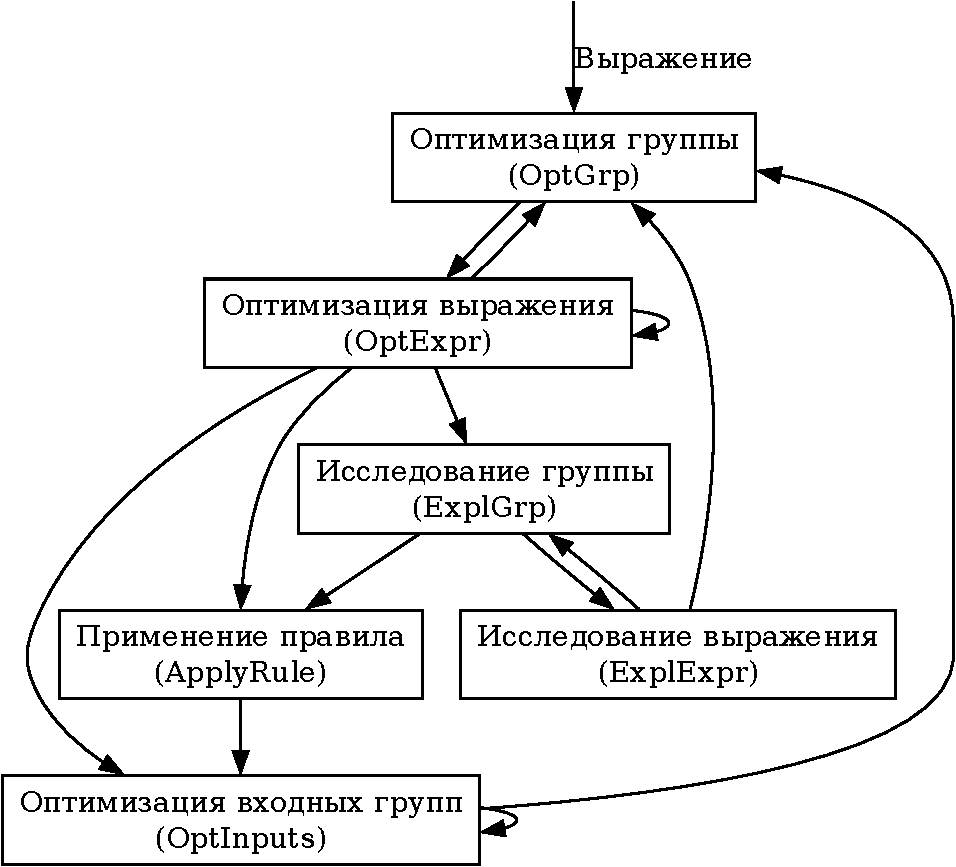
\includegraphics[width=\textwidth,height=0.62\textheight,keepaspectratio]{cascades.pdf}
\end{column}
\end{columns}
\end{frame}

\begin{frame}{Процесс обработки запроса}
\centering
\resizebox{0.88\textwidth}{!}{%
\begin{tikzpicture}[
    scale=0.95, transform shape,
    node/.style={rectangle, draw, rounded corners=2pt,
                 text width=3.0cm, minimum height=0.8cm,
                 align=center, font=\scriptsize},
    main/.style={node, fill=gray!8},
    io/.style={node, fill=gray!20},
    aux/.style={node, dashed},
    arrow/.style={-{Stealth[length=2.5mm]}, thick},
    auxarrow/.style={-{Stealth[length=2.5mm]}, thick, dashed}
]
    \node[io]   (sql)    at (0, 0) {Генератор\\случайных\\запросов};
    \node[main] (parse)  at (0, -2) {Разбор};
    \node[main] (optim)  at (0, -4.5) {Оптимизация\\ и\\проверка\\ достижимости};
    \node[main] (exec)   at (0, -6.65) {Исполнение};
    \node[io]   (result) at (0, -8.2) {Результат};

    \node[aux] (mssqlplan) at (5.0, -1.55) {MSSQL};
    \node[aux] (diff)      at (5.0, -4.65) {Проверка\\корректности};
    \node[aux] (mssqlres)  at (-5.0, -1.55) {MSSQL};
    \node[aux] (reach)     at (-5.0, -4.5) {Конвертация\\в план\\модельной СУБД};

    \draw[arrow] (sql) -- node[right, font=\scriptsize] {запрос} (parse);
    \draw[arrow] (parse) -- node[right, font=\scriptsize] {реляционная алгебра} (optim);
    \draw[arrow] (optim) -- node[right, font=\scriptsize] {план} (exec);
    \draw[arrow] (exec) -- (result);

    \draw[auxarrow] (sql) -- node[above, font=\scriptsize] {запрос} (mssqlplan);
    \draw[auxarrow] (mssqlplan) -- node[right, font=\scriptsize] {результат} (diff);
    \draw[auxarrow] (result.east) -- ++(1.2,0) |- (diff.west);

    \draw[auxarrow] (sql) -- node[above, font=\scriptsize] {запрос} (mssqlres);
    \draw[auxarrow] (mssqlres) -- node[left, font=\scriptsize] {план} (reach);
    \draw[auxarrow] (reach.east) -- node[above, font=\scriptsize] {планы} (optim.west);
\end{tikzpicture}
}
\end{frame}

\begin{frame}{Реляционная алгебра}
\begin{itemize}
  \item \(\sigma_p(E)\) --- фильтрация кортежей по предикату \(p\).
  \item \(\pi_{\bar a}(E)\) --- проекция выбранных атрибутов.
  \item \(E_1 \times E_2\) --- декартово произведение отношений.
  \item \(E_1 \Join_p E_2\) --- соединение отношений по предикату.
  \item \(\gamma_{\bar g;\bar f}(E)\) --- группировка и вычисление агрегатов.
  \item \(\tau_{\bar a}(E)\) --- сортировка результата.
\end{itemize}

\begin{block}{Форма запроса}
\[
  \Projection{\bar a}{\Sel{p}{E_1 \times \ldots \times E_n}},
  \qquad
  \Agg{\bar g}{\bar f}{\Sel{p}{E_1 \times \ldots \times E_n}}
\]
\end{block}
\end{frame}

\begin{frame}{Правила оптимизации}
\footnotesize
\begin{columns}[T,onlytextwidth]
\begin{column}{0.54\textwidth}
\begin{block}{Трансформации}
\begin{itemize}
  \item коммутативность и ассоциативность соединений;
  \item разбиение, объединение и проталкивание фильтров;
  \item проталкивание проекций через соединение;
  \item преобразование \sqlkw{IN} в цепочку сравнений;
  \item перенос фильтра в предикат соединения;
  \item внешнее соединение во внутреннее;
  \item проталкивание и перестановка агрегации.
\end{itemize}
\end{block}
\end{column}
\begin{column}{0.42\textwidth}
\begin{block}{Реализации}
\begin{itemize}
  \item \SeqScan, \IndexScan;
  \item \sqlkw{Filter}, \sqlkw{Projection};
  \item \NestedLoopJoin, \HashJoin, \MergeJoin;
  \item \sqlkw{HashAggregate};
  \item \sqlkw{StreamAggregate}.
\end{itemize}
\end{block}
\end{column}
\end{columns}
\end{frame}

\begin{frame}{Стоимостная модель}
\begin{block}{Отсечение ветвей}
Если для группы \(G\) и свойства \(P\) уже найден план стоимости \(C^*\), то
физическое выражение \(e\) можно не рассматривать при выполнении условия:
\[
  C_{local}(e) + \sum_{i=1}^{k} LB(G_i, P_i) \geq C^*.
\]
\end{block}

\begin{center}
\scriptsize
\begin{tabular}{@{}ll@{}}
\toprule
Физический оператор & Формула стоимости \\
\midrule
Последовательное сканирование & \(100\,n\) \\
Проекция & \(22\,n_{out}\) \\
Сортировка & \(11\,n(\lfloor\log_2 n\rfloor + 1)\) \\
Агрегация & \(510\,n\) \\
Потоковая агрегация & \(130\,n\) \\
Соединение вложенными циклами & \(70\,n_l n_r\) \\
Декартово произведение & \(104\,n_l n_r\) \\
\bottomrule
\end{tabular}
\end{center}
\end{frame}

\begin{frame}{Дифференциальный анализ планов}
\begin{block}{Основная идея}
  Проверяем, достижим ли план, построенный промышленной СУБД, при текущем наборе
  правил и условиях активации. Цель: найти недостающие правила и уточнить
  правила активации.
\end{block}

\begin{enumerate}
  \item Генерируется случайный SQL-запрос из поддерживаемого подмножества.
  \item Microsoft SQL Server строит физический план.
  \item ShowPlanXML конвертируется во внутренний формат проекта.
  \item Запускается оптимизатор с отключенным B\&B.
  \item Структурно соотносится получившееся пространство поиска и эталонный план.
\end{enumerate}
\end{frame}

\begin{frame}[fragile]{Пример найденного расхождения}
\begin{lstlisting}
SELECT markets.id AS c2619
FROM markets CROSS JOIN users CROSS JOIN books
WHERE markets.region != 'AMERICA';
\end{lstlisting}

\begin{columns}[T,onlytextwidth]
\begin{column}{0.49\textwidth}
\centering
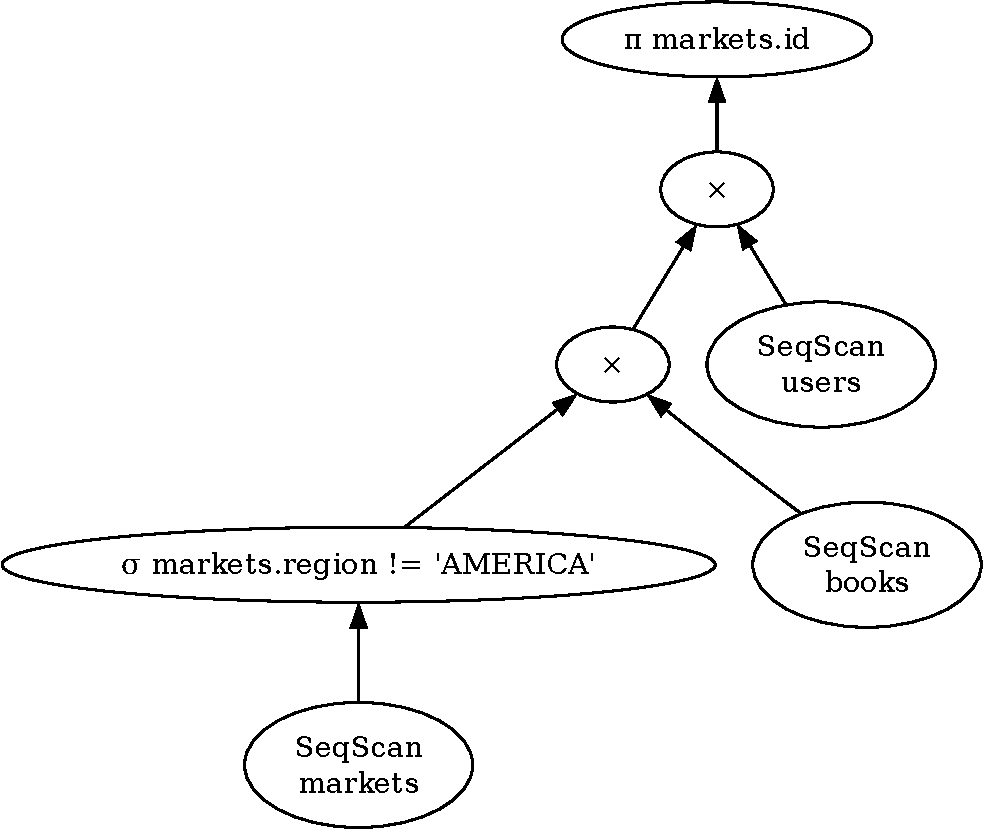
\includegraphics[width=\textwidth,height=0.42\textheight,keepaspectratio]{reach-fuzz-cross-mssql.pdf}

\scriptsize План Microsoft SQL Server
\end{column}
\begin{column}{0.49\textwidth}
\centering
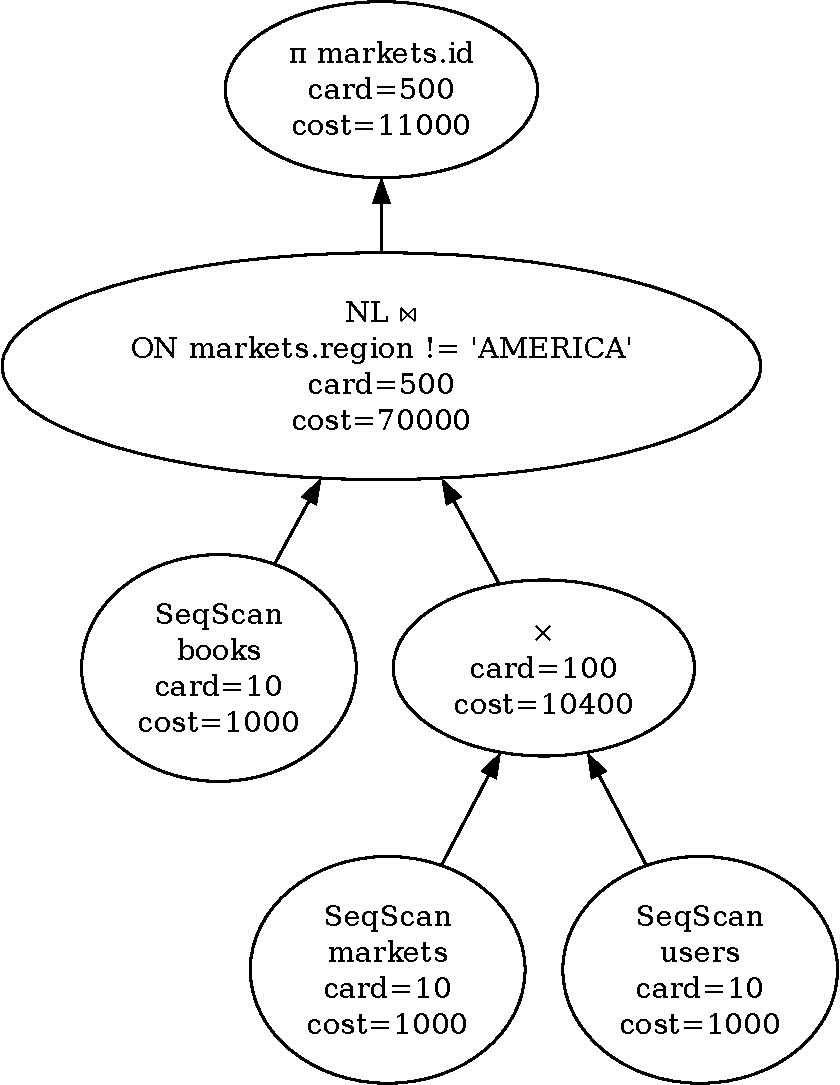
\includegraphics[width=\textwidth,height=0.42\textheight,keepaspectratio]{reach-fuzz-cross-ours.pdf}

\scriptsize План модельной СУБД
\end{column}
\end{columns}
\end{frame}

\begin{frame}{Результаты проверки пространства поиска}
\begin{center}
\small
\begin{tabular}{@{}lr@{}}
\toprule
Показатель & Значение \\
\midrule
Количество сгенерированных запросов & 1000 \\
Достижимый план промышленной СУБД & 251 \\
Недостижимый план промышленной СУБД & 244 \\
Пропущено & 505 \\
Ошибки преобразования плана & 496 \\
Ошибки преобразования из-за исключений & 9 \\
Ошибки получения плана Microsoft SQL Server & 0 \\
Среднее расстояние до ближайшего плана & 2.37 \\
\bottomrule
\end{tabular}
\end{center}

  \begin{itemize}
    \item 25\% от общего числа планов совпали.
    \item 25\% требуют уточнения правил.
    \item 50\% требуют расширения набора операторов.
  \end{itemize}
\end{frame}

\begin{frame}{Производительность}
\centering
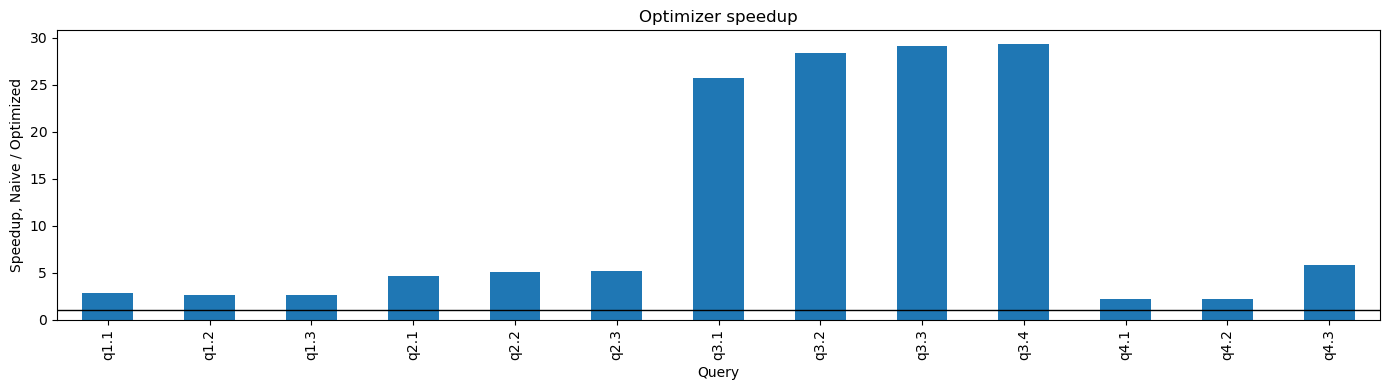
\includegraphics[width=\textwidth,height=0.50\textheight,keepaspectratio]{optimizer-speedup.png}

\raggedright
\begin{itemize}
  \item Сравнивались режимы \texttt{Naive} и \texttt{Optimized}.
  \item Использованы запросы Star Schema Benchmark.
  \item На выбранном наборе тестов получено ускорение \(2.5\text{--}30\) раз.
\end{itemize}
\end{frame}

\begin{frame}{Калибровка стоимостной модели}
\begin{columns}[T,onlytextwidth]
\begin{column}{0.49\textwidth}
\centering
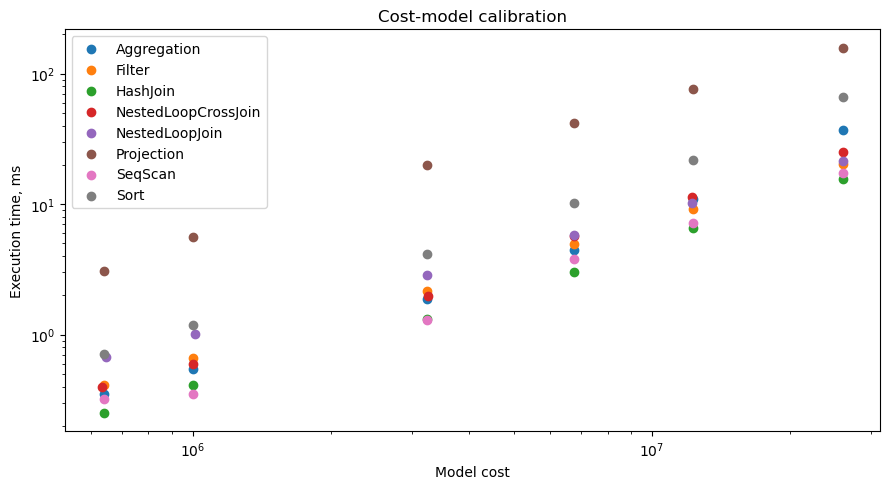
\includegraphics[width=\textwidth,height=0.40\textheight,keepaspectratio]{calibration.png}

\scriptsize Физические операторы
\end{column}
\begin{column}{0.49\textwidth}
\centering
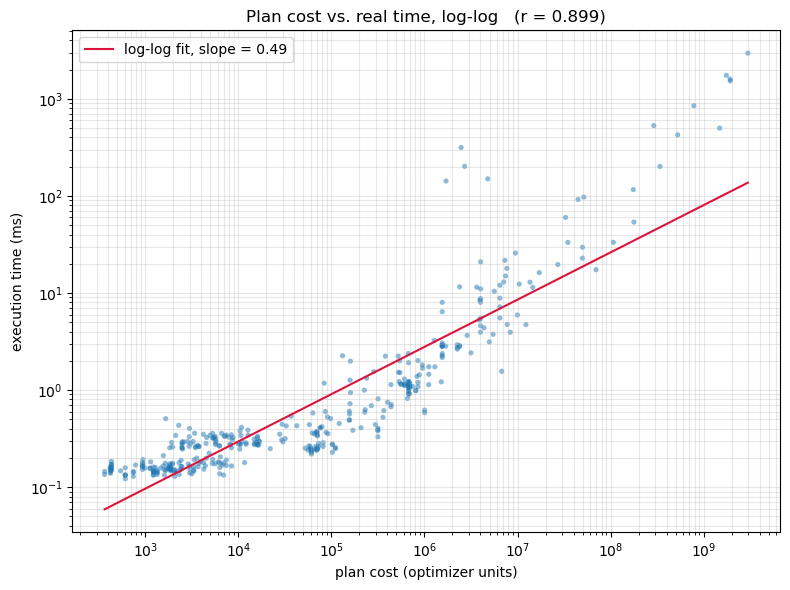
\includegraphics[width=\textwidth,height=0.40\textheight,keepaspectratio]{cost-on-random-queries.png}

\scriptsize Случайные запросы
\end{column}
\end{columns}

\footnotesize
\begin{itemize}
  \item Формулы стоимости откалиброваны по бенчмаркам физических операторов.
  \item Общая стоимость планов согласована с реальным временем исполнения.
\end{itemize}
\end{frame}

\end{document}
